% Copyright 2015, 2016 Dustin Lang (U Toronto).
% All rights reserved.

% TO-DO:
% - Journal reference for Peterson
% - think carefully about ``convolution'' vs ``correlation''

% - provide exp and deV GMM parameters in an appendix?

% - provide the model space to pixel space (ellipse and WCS
%   transformation) equations?

% - discuss wrap-around and required pixel stamp size

\documentclass[11pt,preprint]{aastex}
\usepackage{amssymb,amsmath,mathrsfs,color}
\usepackage{bm}
\usepackage{hyperref}
\usepackage{multirow}
\usepackage{color}

\hypersetup{pdftitle={},
pdfauthor={Dustin Lang},pdfsubject={Astronomical image processing}}

\newcommand{\arxiv}[1]{\href{http://arxiv.org/abs/#1}{arXiv:#1}}

\newcommand{\foreign}[1]{\emph{#1}}
\newcommand{\etal}{\foreign{et\,al.}}
\newcommand{\ie}{\foreign{i.e.}}
\newcommand{\figref}[1]{\figurename~\ref{#1}}
\newcommand{\Figref}[1]{\figref{#1}}
\newcommand{\niceurl}[1]{\href{#1}{\textsl{#1}}}
\newcommand{\project}[1]{\textsl{#1}}
\newcommand{\conv}{\otimes}
\newcommand{\trick}{method}
\newcommand{\Trick}{Method}

\definecolor{gray}{rgb}{0.5,0.5,0.5}
\newcommand{\gray}[1]{\textcolor{gray}{#1}}

\slugcomment{Submitted to The Astronomical Journal}

\keywords{methods: data analysis --- surveys --- techniques: image processing}

\begin{document}

\title{A \trick\ for fast galaxy--PSF convolution}
\author{Dustin~Lang\altaffilmark{1,2,3}}
%\email{dstndstn@gmail.com}
%\affil%
\altaffiltext{1}%
{Department of Astronomy \& Astrophysics and Dunlap Institute,
  University of Toronto,
  50 Saint George Street, Toronto, ON, M5S 3H4, Canada}
%\\ and
\altaffiltext{2}%
{Department of Physics \& Astronomy,
  University of Waterloo,
  200 University Avenue West,
  Waterloo, ON, N2L 3G1, Canada}
\altaffiltext{3}%
{dstndstn@gmail.com}
\date{}
\shorttitle{Fast Galaxy--PSF Convolution}
\shortauthors{Lang}

\begin{abstract}
  I present a \trick\ for the fast convolution of a model galaxy profile
  by a point-spread function (PSF) model that can be represented in
  the Fourier domain.  The \trick\ relies upon two observations: First, most
  simple galaxy profiles of common interest (deVaucouleurs,
  exponential, S\'ersic) can be approximated as mixtures of Gaussians.
  Second, the Fourier transform of a Gaussian is a Gaussian, thus the
  Fourier transform of a mixture-of-Gausssian approximation of a
  galaxy can be directly evaluated in Fourier space.  This \trick\ 
  allows the use of pixelized PSF models (ie, a PSF represented as a
  grid of pixel values) in galaxy model-fitting approaches such as
  \project{the Tractor}.
\end{abstract}

\section{Introduction}

A number of codes exist to render images of galaxies as they would
appear when observed with a (real or imagined) telescope and camera,
and given observing conditions (sky brightness, atmosphere).  These
include \project{GalSim} \citep{galsim}, \project{Ufig} \citep{ufig},
\project{phosim} \citep{phosim}, \project{galfit} \citep{galfit}, 
\project{the Tractor} (Lang \etal, in prep), and several others.

%\project{MegaMorph} \citep{megamorph}, 

In codes that simulate at the pixel level rather than the photon
level, it is necessary to convolve a galaxy's appearance ``above the
atmosphere'' (at high resolution and before any effects from the
atmosphere, optics, or detector) by the point-spread function to
produce the image as it would appear on the CCD.  This step often
dominates the computation time required to render a galaxy.  Since
model galaxy profiles such as the deVaucouleurs profile are very
``peaky'', typical galaxy images ``above the atmosphere'' are
undersampled by the native resolution of the CCD.  Thus it is not
possible to render na\"ively the above-the-atmosphere galaxy at native
pixel scale and then convolve by the PSF (also represented at native
pixel scale).  Codes typically attempt to render the images at higher
resolution than the CCD pixels and then bin down to the native CCD
resolution; this significantly increases the computational cost, and
may still not achieve exactly correct results.

In \project{the Tractor}, we have previously taken the approach of
using mixture-of-Gaussian approximations for \emph{both} the PSF and
the model galaxy profiles.  The galaxy profile approximations are
presented in \cite{moggalaxy}.  With the PSF and galaxy represented as
mixtures of Gaussians, convolution is analytic and results in a larger
mixture of Gaussians (the product of the two mixture sizes), which can
then be directly evaluated.  This approach has the distinct limitation
that the PSF must be approximated as a mixture of Gaussians; in
practice, it takes many Gaussians to achieve a good approximation, and
this makes the computation expensive.

\section{The \Trick}

The \trick\ builds directly upon our mixture-of-Gaussians
approximation of galaxy profiles, with the realization that the
Fourier transform of a Gaussian is also a Gaussian.  This allows us to
evaluate the Fourier transform of a galaxy \emph{directly} in Fourier
space, without ever having to render the ``above the atmosphere''
(unconvolved) galaxy profile in pixel space (which is problematic due
to undersampling).  We can then multiply this Fourier-space
representation of the galaxy by the Fourier transform of the pixelized
PSF model, then inverse Fourier transform back to pixel space to get
the PSF-convolved galaxy profile.

The method, then, is:
\begin{enumerate}
\item Choose the desired output image size and embed the pixelized PSF
  model in a zero-padded image of this size.
\item Compute the Fourier Transform of the padded PSF model via the
  Fast Fourier Transform (FFT),
  recording the frequencies $(v, w)$ of the FFT terms.
\item Transform the mixture-of-Gaussians approximation of the model
  galaxy through an ellipticity matrix and the local image World
  Coordinate System (WCS) matrix to get pixel-space Gaussians.
\item Convert the galaxy mixture-of-Gaussians from pixel space to Fourier space.
\item Evaluate the Fourier-space Gaussians on the frequency grid $(v, w)$.
\item Multiply the PSF and galaxy Fourier transforms and inverse-FFT
  back to pixel space.
\end{enumerate}

\begin{figure}
  \newcommand{\arrowspacer}[1]{\left#1 \textrm{\rule[-0.5em]{0pt}{1em}} \right.}
  \begin{center}
    \begin{tabular}{@{}ccc@{}}
      %
      PSF & \gray{Galaxy} & Result: PSF $\conv$ Galaxy \\
      % psf img
      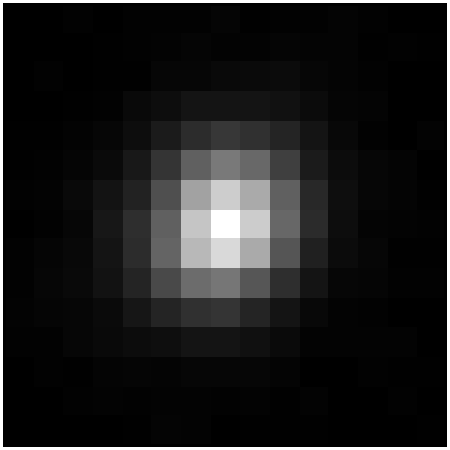
\includegraphics[height=0.22\textwidth]{psf-00} &
      % gal img*
      \includegraphics[height=0.22\textwidth]{psf-04} &
      % psf * gal img
      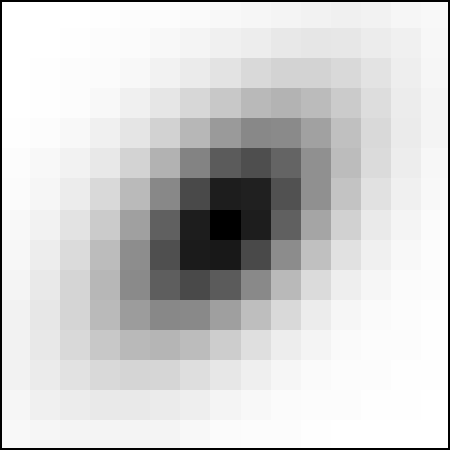
\includegraphics[height=0.22\textwidth]{psf-05} \\
      %
      \rule[-1em]{0pt}{1.5em}
      $\arrowspacer{\downarrow}$ & & $\arrowspacer{\uparrow}$ \\
      %
      FFT(PSF) & FT(Galaxy) & FFT(PSF) * FT(Galaxy) \\
      % psf FT
      \multicolumn{1}{r}{%
        \includegraphics[height=0.22\textwidth]{psf-01}} &
      % gal FT
      \multicolumn{1}{r}{%
        \includegraphics[height=0.22\textwidth]{psf-02}} &
      % psf * gal FT
      \multicolumn{1}{r}{%
        \includegraphics[height=0.22\textwidth]{psf-03}}
      % gal img
      %\includegraphics[height=0.22\textwidth]{psf-12} &
    \end{tabular}
  \end{center}
  \caption{\label{fig:example}
    Illustration of the \trick.
    \textbf{Top-left}: pixelized PSF model.
    %
    \textbf{Bottom-left}: FFT of the pixelized PSF model.  Since the PSF model is
    purely real, we show only half the symmetric Fourier transform; the FFT is
    complex; we show here the absolute value.
    % 
    \textbf{Top-middle}: pixel-space galaxy profile (which would be
    undersampled), with Gaussian ellipse approximations.  This is
    never evaluated in our method, and is shown only for illustration.
    % 
    \textbf{Bottom-middle}: the discrete Fourier-space representation of the
    galaxy profile, evaluated directly in Fourier space.
    %
    \textbf{Bottom-right}: product of the FFT of the PSF and the
    discrete Fourier transform of the galaxy model.
    %
    \textbf{Top-right}: the result: the galaxy model convolved by the
    PSF, in pixel space.  This is computed by inverse-FFT of the
    bottom-right panel.
  }
\end{figure}

Step 1, choosing the desired output image size, depends on the size of
the PSF model as well as the galaxy.  If the chosen size is too small,
wrap-around will occur since the FFT is periodic.

In Step 3, we transform the mixture-of-Gaussians approximation of the
galaxy profiles from their representation in units of galaxy effective
radius into pixel units.  This includes an ellipse transformation
(scaling by effective radius, shearing by galaxy axis ratio, rotation
by galaxy position angle), plus a transformation into pixel
coordinates based on a locally-linear approximation of the image's
World Coordinate System.
% We split the pixel position of the galaxy center into integer and
% fractional parts.
The result is a pixel-space mixture-of-Gaussians representation of the
galaxy.

Step 4 is the core of the \trick.  The Fourier transform of
a Gaussian is another Gaussian; our mixture-of-Gaussian representation
of galaxy profiles can be converted into a mixture of Gaussians in
Fourier space.
%
A single 2-dimensional Gaussian
centered at the origin and
with covariance $C$
in pixel space is defined by
\begin{equation}
g(\bm{x}) = \frac{1}{2 \pi \sqrt{\det(C)}}
\exp\left( -\frac{1}{2} \bm{x}^T C^{-1} \bm{x} \right)
\end{equation}
which becomes, writing out the vector $\bm{x}$ as $(x,y)^T$
and covariance $C = \bigl(\begin{smallmatrix}
a&b \\ b&d
\end{smallmatrix} \bigr)$,
\begin{equation}
g(x, y) = \frac{1}{2 \pi \sqrt{a d - b^2}}
\exp \left(
-\frac{d x^2 - 2 b x y + a y^2}{2(a d - b^2)}
\right) \quad .
\end{equation}
%
The Fourier Transform of the shifted Gaussian $g(x - x_0, y - y_0)$ is defined as
\begin{equation}
G(v,w) =
\int\limits_{-\infty}^{\infty}
\int\limits_{-\infty}^{\infty}
g(x - x_0, y - y_0) e^{-2 \pi i (v x + w y)} \, \mathrm{d}x \, \mathrm{d}y
\quad .
\end{equation}
We use the shift theorem to move the centroid to $\mu = (x_0, y_0)$
in pixel space via a phase term in Fourier space;
\begin{equation}
G(v, w) =
e^{-2 \pi i (x_0 v + y_0 w)}
\int\limits_{-\infty}^{\infty}
\int\limits_{-\infty}^{\infty}
g(x, y) e^{-2 \pi i (v x + w y)} \, \mathrm{d}x \, \mathrm{d}y
\end{equation}
%
which, plugging in the covariance matrix $C$, works out to
\begin{equation}
G(v,w) =
e^{-2 \pi i (x_0 v + y_0 w)}
e^{-2 \pi^2 (a v^2 + 2 b v w + d w^2)}
\end{equation}
which can easily be evaluated on a grid of frequencies $(v, w)$.

For a mixture of Gaussians, we must evaluate $G$ for each component in
the mixture and compute their weighted sum.  In the case of a
mixture-of-Gaussians representation of affine-transformed galaxy
profiles, the centers $(x_0, y_0)$ are the same for each component in
the mixture; only the covariances,
$C_i = \bigl(\begin{smallmatrix}
a_i&b_i \\ b_i&d_i
\end{smallmatrix} \bigr)$,
differ.  The Fourier transform
of a mixture of Gaussians,
\begin{equation}
m(x,y) = \sum_i A_i \, g_i(x, y)
\end{equation}
is therefore
\begin{equation}
M(v, w) = e^{-2 \pi i (x_0 v + y_0 w)}
\sum_i A_i \,
e^{-2 \pi^2 (a_i v^2 + 2 b_i v w + d_i w^2)}
\quad .
\end{equation}



%%% Example of pushing our galaxy MOGs through a WCS, etc?


Then, in Step 5, we directly evaluate these Gaussians in Fourier
space, on the same discrete frequency grid $(v, w)$ used for the FFT
of the PSF.  This has interesting properties.  By taking the Fourier
transform, we are effectively assuming that the PSF model is well
sampled, thus has zero power outside the frequency grid of the FFT.
The galaxy profile may have power outside that frequency range; this
is the reason that one cannot simply render the galaxy profile ``above
the atmosphere'' at the native image pixel scale and apply FFT
convolution na\"ively; In the limit, a point-like galaxy has power at
all frequencies.  But when we multiply the PSF and galaxy profile in
Fourier space, all that high-frequency power will be zeroed out by the
assumption of well-sampled PSF model.  Effectively, by evaluating the
galaxy Fourier transform directly in the frequency space of the PSF
model, we are applying a perfect low-pass filter at exactly the
Nyquist limit.  By zeroing out the high-frequency power, we avoid the
aliasing that would otherwise result from Fourier transforming an
undersampled signal.
%

Finally, in Step 6, we multiply the PSF and galaxy Fourier transforms,
and apply the inverse FFT to return to pixel space.

Figure \ref{fig:example} illustrates this process.

\section{Discussion}

--implemented in The Tractor

--speed \& accuracy example vs GMM

--efficiency with PsfEx-style eigen-PSF models

--choosing patch size...


\section{Conclusion}





\begin{thebibliography}

\bibitem[Berg\'e \etal(2013)]{ufig}
Berg\'e,~J. \etal, 2013, Astronomy and Computing, 1, 23;
\arxiv{1209.1200}
% An Ultra Fast Image Generator (UFig) for wide-field astronomy

\bibitem[Hogg \& Lang(2013)]{moggalaxy}
Hogg,~D.~W. \and Lang,~D., 2013, \pasp, 125, 719;
\arxiv{1210.6563}

% Detailed Structural Decomposition of Galaxy Images
\bibitem[Peng \etal(2002)]{galfit}
 Peng,~C.~Y. \etal, 2002, \aj, 124, 266;
 \arxiv{0204182}

% PhoSim: a code to simulate telescopes one photon at a time
%Peterson,~J.~R., 2014, Journal of Instrumentation, 9, C04010;
%Simulation of Astronomical Images from Optical Survey Telescopes using a Comprehensive Photon Monte Carlo Approach
\bibitem[Peterson \etal(2015)]{phosim}
Peterson,~J.~R. \etal, 2015, 218, 14;
\arxiv{1504.06570}

\bibitem[Rowe \etal(2015)]{galsim}
  Rowe,~B. \etal, 2015, Astronomy and
  Computing, 10, 121; \arxiv{1407.7676}
% GalSim: The modular galaxy image simulation toolkit

\end{thebibliography}


\end{document}
